% The maps and the single-city figures for the Module 1 sheet, kept in their
% own file because the answer key draws exactly the same maps with the
% circles filled in. Needs tikz, its calc and positioning libraries, and the
% colour pltblue, all of which the including file sets up.
% ---------------------------------------------------------------------------
% The map: seven Upstate New York highways over four cities. The cities sit
% where they really sit --- Ithaca west, Syracuse north, Binghamton south,
% Albany far east --- and every road on it is a road you can drive, so the
% figure reads as a road map rather than as an abstract graph. The degrees are
% Ithaca 3, Syracuse 4, Binghamton 4, Albany 3; US-11, on the second copy,
% takes Syracuse and Binghamton to 5.
%
% \nymap{extra roads}{numbers already filled in}. The route is written on the
% map, not copied out as letters: each road carries a circle, and the order it
% is driven goes in the circle.
% ---------------------------------------------------------------------------
\tikzset{
  % Every road is drawn the same, so no line weight or colour suggests a
  % distinction that isn't there. Only the shields differ, as on a real map.
  road/.style     = {line width=3.6pt, black!62, line cap=round},
  ishield/.style  = {draw=pltblue!60!black, fill=pltblue, text=white,
                     font=\bfseries\scriptsize, rounded corners=1.6pt,
                     inner sep=2pt},
  nshield/.style  = {draw=black!65, fill=white, text=black,
                     font=\bfseries\scriptsize, rounded corners=1.6pt,
                     inner sep=2pt},
  city/.style     = {circle, fill=black, inner sep=0pt, minimum size=6.5pt},
  cityname/.style = {font=\bfseries, inner sep=3pt},
  % The circle a student writes the order into, and the pre-filled number.
  ord/.style      = {circle, draw=pltblue!75, line width=0.7pt, fill=white,
                     minimum size=0.44cm, inner sep=0pt},
  ordnum/.style   = {font=\bfseries\footnotesize, inner sep=0pt},
}
\newcommand{\nymap}[2]{%
\begin{tikzpicture}[x=0.88cm, y=0.88cm]
    \begin{scope}
        \clip (0,0) rectangle (13,7.0);
        \fill[black!3] (0,0) rectangle (13,7.0);
        \fill[pltblue!22] (0,5.0) .. controls (1.8,6.0) and (2.6,6.5) ..
                          (5.0,7.0) -- (0,7.0) -- cycle;
    \end{scope}
    \node[font=\itshape\scriptsize, black!45, rotate=20] at (1.6,6.0)
        {Lake Ontario};

    \coordinate (I) at (1.8,2.3);
    \coordinate (S) at (5.0,5.9);
    \coordinate (B) at (4.4,0.9);
    \coordinate (A) at (11.6,3.3);

    \draw[road] (I) to[bend left=28]  (S);
    \draw[road] (I) to[bend right=26] (S);
    \draw[road] (I) to[bend right=8]  (B);
    \draw[road] (S) to[bend left=12]  (B);
    \draw[road] (S) to[bend left=8]   (A);
    \draw[road] (B) to[bend left=11]  (A);
    \draw[road] (B) to[bend right=11] (A);
    #1

    % Shields on a second pass, so no road is drawn across a number. Each
    % carries its circle as a label, on whichever side is clear of other roads.
    \path (I) to[bend left=28]  node[nshield, pos=0.55,
          label={[ord, name=o34]180:{}}] {NY-34} (S);
    \path (I) to[bend right=26] node[nshield, pos=0.35,
          label={[ord, name=o13]0:{}}]   {NY-13} (S);
    \path (I) to[bend right=8]  node[nshield, pos=0.50,
          label={[ord, name=o79]180:{}}] {NY-79} (B);
    \path (S) to[bend left=12]  node[ishield, pos=0.72,
          label={[ord, name=o81]90:{}}]  {I-81}  (B);
    \path (S) to[bend left=8]   node[ishield, pos=0.46,
          label={[ord, name=o90]90:{}}]  {I-90}  (A);
    \path (B) to[bend left=11]  node[ishield, pos=0.50,
          label={[ord, name=o88]90:{}}]  {I-88}  (A);
    \path (B) to[bend right=11] node[nshield, pos=0.50,
          label={[ord, name=o7]270:{}}]  {NY-7}  (A);

    \node[city] at (I) {};  \node[cityname, below left] at (I) {Ithaca};
    \node[city] at (S) {};  \node[cityname, above] at (S) {Syracuse};
    \node[city] at (B) {};  \node[cityname, below] at (B) {Binghamton};
    \node[city] at (A) {};  \node[cityname, above] at (A) {Albany};

    \draw[->, black!50, line width=1pt] (12.4,5.6) -- (12.4,6.35);
    \node[font=\bfseries\footnotesize, black!50] at (12.4,6.65) {N};
    \draw[black!35] (0,0) rectangle (13,7.0);
    #2
\end{tikzpicture}}

% US-11, the eighth road on the second copy. It really does run beside I-81,
% but it is bowed east far enough that both roads, and both shields, are
% legible; the shield is nudged clear of I-81's lane.
\newcommand{\usroad}{%
    \draw[road] (S) to[bend left=40] (B);
    \path (S) to[bend left=40] node[nshield, pos=0.50, xshift=17pt,
          label={[ord, name=o11]0:{}}] {US-11} (B);}

% ---------------------------------------------------------------------------
% One city on its own, with #1 road-ends radiating out. #2 takes extra TikZ so
% the k=2 figure can ship with its pairing already drawn.
% ---------------------------------------------------------------------------
\newcommand{\landdeg}[2]{%
\begin{tikzpicture}[x=1cm, y=1cm]
    \path (-1.55,-1.55) rectangle (1.55,1.55);
    \foreach \i in {1,...,#1} {
        \pgfmathsetmacro\ang{90 - (\i-1)*360/#1}
        \draw[line width=2.6pt, black!72] (\ang:0.38) -- (\ang:1.18);
        \draw[thick, fill=white] (\ang:1.28) circle (0.1);
    }
    \draw[thick, fill=white] (0,0) circle (0.38);
    #2
\end{tikzpicture}}

% ---------------------------------------------------------------------------
% The three graphs the sheet asks about after the map: Konigsberg as Euler
% drew it, the five bus stops, and the four-node network Part 3 predicts.
% ---------------------------------------------------------------------------
\newcommand{\konigsberggraph}{%
\begin{tikzpicture}[x=0.72cm, y=0.72cm, thick,
                    every node/.style={draw, circle, minimum size=0.85cm,
                                       inner sep=1pt, fill=white}]
    \node (C) at (0,2.5)   {C};
    \node (A) at (0,0)     {A};
    \node (B) at (0,-2.5)  {B};
    \node (D) at (3.4,0)   {D};
    \draw (A) to[bend left=32]  (B);
    \draw (A) to[bend right=32] (B);
    \draw (A) to[bend left=32]  (C);
    \draw (A) to[bend right=32] (C);
    \draw (A) -- (D);
    \draw (B) -- (D);
    \draw (C) -- (D);
    \node[draw=none, fill=none, pltblue] at (-1.15,-1.25) {\emph{a}};
    \node[draw=none, fill=none, pltblue] at ( 1.15,-1.25) {\emph{b}};
    \node[draw=none, fill=none, pltblue] at (-1.15, 1.25) {\emph{c}};
    \node[draw=none, fill=none, pltblue] at ( 1.15, 1.25) {\emph{d}};
    \node[draw=none, fill=none, pltblue] at ( 1.75, 0.45) {\emph{e}};
    \node[draw=none, fill=none, pltblue] at ( 2.25,-1.5)  {\emph{f}};
    \node[draw=none, fill=none, pltblue] at ( 2.25, 1.5)  {\emph{g}};
\end{tikzpicture}}

\newcommand{\busstopgraph}{%
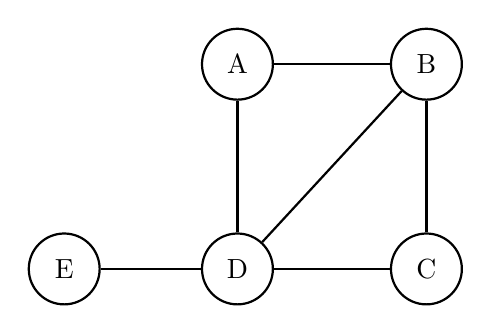
\begin{tikzpicture}[x=1cm, y=1cm, thick,
                    every node/.style={draw, circle, minimum size=0.9cm,
                                       inner sep=1pt, fill=white}]
    \node (A) at (0,1.6)   {A};
    \node (B) at (2.4,1.6) {B};
    \node (C) at (2.4,-1)  {C};
    \node (D) at (0,-1)    {D};
    \node (E) at (-2.2,-1) {E};
    \draw (A) -- (B);
    \draw (B) -- (C);
    \draw (C) -- (D);
    \draw (D) -- (A);
    \draw (B) -- (D);
    \draw (D) -- (E);
\end{tikzpicture}}

\newcommand{\fournodegraph}{%
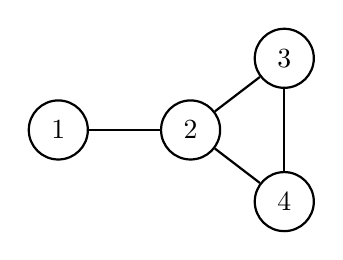
\begin{tikzpicture}[x=0.7cm, y=0.7cm, thick,
                    every node/.style={draw, circle, minimum size=0.75cm,
                                       inner sep=1pt, fill=white}]
    \node (1) at (-2.4,0)  {1};
    \node (2) at (0,0)     {2};
    \node (3) at (1.7,1.3) {3};
    \node (4) at (1.7,-1.3){4};
    \draw (1) -- (2);
    \draw (2) -- (3);
    \draw (2) -- (4);
    \draw (3) -- (4);
\end{tikzpicture}}
